\documentclass{bmstu}

\usepackage{hyperref}

\bibliography{biblio.bib}

\begin{document}
\makethesistitle
{Информатика и системы управления} % Название факультета
{Программное обеспечение ЭВМ и информационные технологии} % Название кафедры
{Автоматическое извлечение ключевых слов и словосочетаний из единичного электронного документа русском языке} % Тема работы
{ИУ7-86Б} % Номер группы
{Барсуков~Н.~М.} % ФИО студента
{Барышникова~М.~Ю.} % ФИО научного руководителя
{Строганов~Ю.~В.} % ФИО консультанта (необязательный аргумент)
{} 
{Мальцева~Д.~Ю.} % ФИО нормоконтролера

\newpage
Задание стр 1
\newpage
Задание стр 2
\newpage
Календарный план
\newpage

\begin{essay}{}
Тема: "Автоматическое извлечение ключевых слов и словосочетаний из единичного электронного документа на русском языке"

Ключевые слова: КС, извлечение ключевых слов, извлечение ключевых словосочетаний, Yake, N-граммы, русский язык, pdf, ключевое слово.

Задачи решаемые в работе:
\begin{enumerate}
	\item анализ существующих методов извлечения ключевых слов;
	\item выбор основного алгоритма и определение направлений его модификации;
	\item проектирование и разработка программного обеспечения для реализации метода;
	\item экспериментальное исследование характеристик разработанного метода;
\end{enumerate}

Область применения разрабатываемого метода -  программные решений в области обработки текстов на естественных языках: поисковые и информационные системы, системы построения авторефератов.

В первой части работы проводится классификация методов извлечения ключевых слов, а так же их обзор.
Во второй части проводится проектирование алгоритма извлечения КС на основе Yake.
В третий части описываются детали реализации разработанного метода.
Четвертая часть посвящена исследованию характеристик разработанного метода.

Поставленная в работе цель было достигнута: был разработ и реализован метод извлечения ключевых слов и словосочетаний из документов на русском языке, проведено исследования характеристик метода и предложены направления дальнейшего развития.
\end{essay}







\maketableofcontents

\begin{definitions}
	\definition{Ключевое слово}{термин из текста описывающий тему документа}
	\definition{Извлечение ключевых слов}{задача по извлечение терминов наилучшем образом описывающих тему документа}
	\definition{PDF}{формат переносимых документов (Portable Document Format)}
	
\end{definitions}
\begin{abbreviations}
	\definition{КС}{ключевое слова}
	\definition{ПО}{программное обеспечение}
	\definition{ИР}{информационная революция}
	\definition{ЯП}{язык программирования}
	\definition{TF}{частота термина (term frequency)}
\end{abbreviations}
\chapter*{ВВЕДЕНИЕ}
\addcontentsline{toc}{chapter}{ВВЕДЕНИЕ}

В истории развития цивилизации выделяют несколько \textbf{информационных революций}.
Первая была связана с изобретением письменности, благодаря чему появилась передача знаний между людьми без непосредственного общения.
Вторая (17-18 вв.) была вызвана благодаря изобретению книгопечатания и реформами школьной системы, сделавшими возможным массовое образование и популяризацию знаний и сыгравшими важную роль в становлении индустриального общества.
Третья и.р. (конец 19 - начало 20 вв.) началась с появлением телеграфа, телефона, радио, позволивших оперативно передавать информацию на любые расстояния и вступила в новую фазу с изобретением телевидения и компьютеров, а затем (кон. 1979-х гг.) с широким распространением информационных технологий. \cite{16}

Количество знаний, накопленных цивилизацией, поражает и, благодаря продолжающейся информационной революции, стремительно растет.
Традиционные медиа, такие как газеты и телевидение, мигрируют в интернет.
Газеты и другие СМИ обновляют новостые ленты в реальном времени, что позволяет интересующимся получать свежую информацию.
Ежедневно милионы пользователей интернета пораждают колоссальное количество контента для различных целей, по разным вопросам, в разных странах, на всевозможных языках и в многообразных онлайн средах.
Это пользовательский контент в блогах и на сайтах социальных сетей, электронная почта, новости, научные работы и т.д.
По всему миру государства, институты, библиотеки, музеи цифвровизируют свои материалы и выкладывают их во всемирную сеть, что бы информацию для бизнеса, науки, исследований, развлечений можно было получить через любое доступное нам "умное" устройство: телефон, планшет, компьютер и т.д. \cite{2}

Таким образом, интернет и стал наиболее эффективными ресурсом для исследования современной экономики, культуры, политики, человеческого общения и взаимодействия людей. \cite{2}

Объемы циркулирующей в мировых телекоммуникационных сетях и хранящейся на серверах информации демонстрируют динамику взрывного роста.
На сегодняшний день, количество опубликованных документов достигает 1 биллиона веб-страниц.
Все указанное обуславливает увеличение состава и сложности программных решений в области обработки текстов на естественных языках в основе которых лежит ряд базовых алгоритмов, в том числе выделения или извлечения ключевых слов (КС).

Извлечение ключевых слов (Keyword extraction) - это задача по автоматическому определению набора терминов, которые наилучшем образом описывают "основную мысль" документа.
При изучении терминов, представляющих наиболее релевантную информацию, содержащуюся в документе, используется различная терминология: ключевые фразы, ключевые сегменты, ключевые термины, или просто ключевые слова.
Однако, несмотря на достаточно большое количество исследований в данной направлении, автоматическое извлечение ключевых слов представляет собой проблему, которая до сих пор не решена \cite{9}. 
Большинство существующих методов, успешно справляющихся с языками с бедной морфологией, такими как английский язык, не пригодны для естественных языков с богатой, в частности для русского языка, где каждая лексема характеризуется большим количеством словоформ с низкой частотностью в каждом конкретном тексте.

Методы способные на извлечения КС из русского языка, представляют в основном своем большинстве объемное программное обеспечение, требующее предварительного сбора и обработки корпуса текстов,  относящихся к одной предметной области, что влечет за собой узконаправленность методов, что ограничивает область применения.

Целью данной работы является разработка метода для автоматического извлечения ключевых слов из электронных документов на русском языке, способного работать с одиночным документом и не зависимого от его предметной области.

Для достижения поставленной цели необходимо выполнить следующие задачи:
\begin{enumerate}
	\item проанализировать современные методы извлечения ключевых слов;
	\item отобрать метод, который будет использоваться в качетсве базового в данной работе и предложить направления его модификации;
	\item описать основные шаги разработанного метода;
	\item разработать программное обеспечение для реализации предложенного метода;
	\item провести эксперементальное сравнение оригинального и модифицированного метода.
\end{enumerate}
\chapter{Аналитический раздел}
В рамках данного раздела представлено описание предметной области задачи по извлечению ключевых слов. 
Приведена систематизация методов извлечения КС и текстов.
Произведен отбор и сравнение методов, удовлетворяющих выставленным ограничениям.
Отобран метод на базе которого будуте производиться модификация.
Определено направление модификации метода.

\section{Задача автоматического извлечения ключевых слов из текста на естественном языке}

Первые попытки теоретического решения проблемы выделения ключевых ("опорных" или "обобщающих") слов была предпринята в работе А.Н. Соколова "Внутренняя речь и мышление" \cite{6}.
Основы современного понимания ключевых слов, можно сформулировать следующим образом \cite{7}:
\begin{enumerate}
	\item ключевые слова отображают тему текста;
	\item их упорядоченность в наборе ключевых слов может трактоваться как эксплицитно невыраженная тема текста;
	\item набор ключевых слов рассматривается как один из минимальных вариантов "текста";
	\item такого типа "текст" характеризуется "ядерной" цельностью и минимальной связностью.
\end{enumerate}

Ключевые слова - это одно или многокомпонентные лексические группы, отражающие содержание документа \cite{3}.

Извлечение ключевых слов (Keyword extraction) - это задача по автоматическому определению набора терминов, которые наилучшим образом описывают объект документа.
При изучении терминов, представляющих наиболее релевантную информацию, содержащуюся в документе, используется различная терминология: ключевые фразы, ключевые сегменты, ключевые термины, или просто ключевые слова.
Все выше перечисленные синонимы имеют одну и туже функцию - охарактеризовать обсуждаемую тему в документе \cite{4}.
Извлечение маленького подмножества элементов, включающих от одного до нескольких терминов из одного документа, является важной проблемой в "Информационном поиске" (Information Retrieval, IR), "Интеллектуальном анализе текста" (Text mining, TM) и в "Обработке естественного языка" (Natural Language Processing, NLP).

Ключевые слова нашли широкое применение в запросах к системам информационного поиска, по сколько их легко определить, пересмотреть, запомнить и поделиться.
По сравнению с математическими сигнатурами, они независимы от любого корпуса и могут применяться в нескольких корпусах и системах ИП \cite{5}.
Так же ключевые слова используются для улучшения функциональности информационно-поисковых систем.
Другими словами они могут быть использованы для создания автоматического индекса для коллекции документов или, в качестве альтернативы, могут использоваться для представления документов в задачах категоризации или классификации \cite{1}.

Общая схема извлечения ключевых слов из текста практически одинакова для всех используемых методов и состоит из следующих шагов:
\begin{enumerate}
	\item предварительная обработка текста:
	\item \begin{enumerate}
		\item исключение элементов маркировки;
		\item приведение слова к словарной форме;
		\item удаление стоп слов, не несущих смысловой нагрузки (предлоги, союзы, частицы, местоимения, междометия и т.д.).
	\end{enumerate}
	\item отбор кандидатов в ключевые слова;
	\item фильтрация кандидатов в ключевые слова (анализ значимых признаков для каждого кандидата).
\end{enumerate}

\section{Систематизация методов}
Доступные публикации описывают классификация методов автоматического извлечения КС разной степени полноты и детализации. 
В самом простом случае исследователи выделяют статистические методы и методы, основанные на машином обучении.
Схожая классификация приводится в работе отечественных авторов, которые рассматривают статистические и гибридные модели КС, на основе которых рассматриваются конкретные методы. 
Более развернутая классификация подразумевает выделение четырех стратегий:
\begin{enumerate}
	\item не требующих обучения; 
	\item простых статистических методов;
	\item лингвистических методов;
	\item метод, основанных на машинном обучении, и их комбинаций.
\end{enumerate}

В последних из доступных отечественных обзоров предметной области извлечения ключевых слов проводится классификация на основе типа системы распознавания которая подразумевает выделение \cite{7}:
\begin{enumerate}
	\item лингвистических;
	\item статистических;
	\item гибридных лингвостатистических метов.
\end{enumerate}

Однако и эта, и прочие классификации не отражают весь спектр и специфику существующих решений.

Так как любой алгоритм извлечения ключевых слов по сути реализует одну или несколько систем распознавания образов, разбивающих входное множество слов на два класса:
\begin{enumerate}
	\item ключевые;
	\item прочие.
\end{enumerate}

то предлагается использовать не иерархическую, а фасетную классификацию соответствующих методов и выбрать следующую совокупность признаков:
\begin{enumerate}
	\item наличие элемента обучения и подходы к его реализации;
	\item тип математического аппарата системы распознавания, обусловленного формой предстваления признаков ключевых слов;
	\item тип используемых для реализации метода лингвистических ресурсов.
\end{enumerate}

По наличию обучения выделяют:
\begin{enumerate}
	\item необучаемые;
	\item обучаемые;
	\item самообучаемые. 
\end{enumerate}
Более простые необучаемые методы подразумевают контекстно независимое выделение КС из отдельного текста на основе априорно составленных моделей и правил. 
Они подходят для гомогенных по функциональному стилю корпусов текстов, увеличивающихся со временем в объемах, на пример научных работ или нормативных актов.
Обучаемые методы предполагают использование разнообразных лингвистических ресурсов для настройки критериев принятия решений при распознавании ключевых слов.
Здесь большое значение имеет корректное выделение КС в выборке, используемой для обучения.
Среди методов с обучением можно выделить подкласс самообучаемых, если обучение ведется без учителя, или с подкрепление на основе пассивной адаптации \cite{20}.

\begin{figure}[h!]
	\centering
	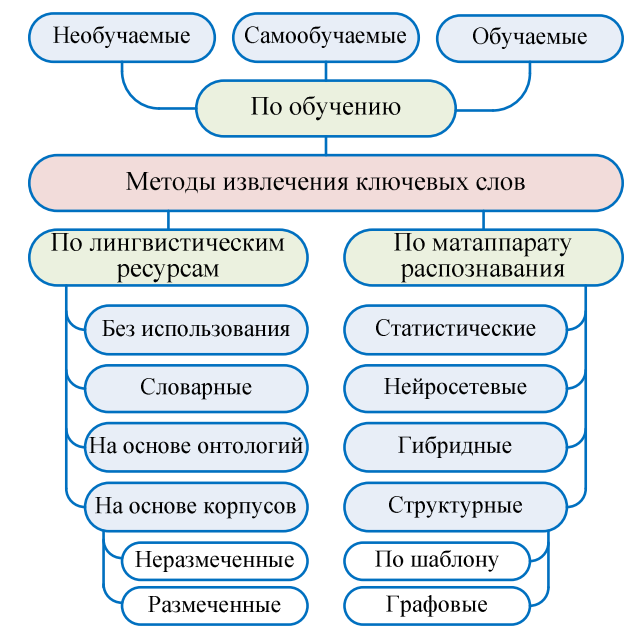
\includegraphics[width=0.7\linewidth]{src/img/ke_types}
	\caption[]{Классификация методов извлечения ключевых слов}
	\label{fig:ketypes}
\end{figure}

По второму признаку классификации прежде всего стоит выделить статистические и структурные методы извлечения КС.
Статистические методы учитывают относительные частоты встречаемости морфологических, лексических, синтаксических единиц и их комбинации.
Это делает создаваемые на их основе алгоритмы довольно простыми, но недостаточно точными, так как признак частотности ключевых слов не является превалирующим.
Одним из классических методов в данном классе является расчет для каждого слова меры, отражающей его важность в тексте, рассматриваемого как элемент коллекции документов.

В основе структурных методов лежит представление о тексте как о системе семантически и грамматически взаимосвязанных элементов слов которые в свою очередь характеризуются набором лингвистических признаков.
Поэтому многие исследователи называют этот класс методов лингвистическим.
Здесь в первом приближении могут быть выделены два подкласса: графовые и синтаксически шаблонные методы.

Графовые или граф-ориентированные методы представляют текс в виде множества слов-вершин или вершин-словосочетаний и ребер отношений между ними.
Эти отношения могут выражать для каждой пары слов такие факты как последовательное появления в тексте, наличие слова в окне заданного размера и семантическую близость.
Для вершин полученного графа вычисляются меры центральности и по пороговому критерию отбираются ключевые слова.
Различия между данными методами состоят в особеностях учета значимости каждой вершины и вычисления отношений между ними.
В основе синтаксических шаблонных методов лежит представление о регулярных синтаксических конструкциях, содержащих на определенных позициях ключевые слова.
В чистом виде такие методы слабо применимы к рассматриваемой задаче, могут использоваться в сочетании с другими.

Нейросетевые методы к задаче извлечения КС стали применяться сравнительно недавно. 
Они основаны на свойстве искуственных нейронных сетей к обобщению и выделению скрытых зависимостей между входными и выходными данными.
Однако для формирования наборов данных для обучения и функционирования нейронных сетей требуется выделение структурных и статистических признаков, поэтому на практике методы выделения КС являются гибридными, т.е. сочетающими в себе элементы основных рассмотренных классов.

Наконец, алгоритмы извлечения КС, реализующие означенные методы, могут не использовать какие либо лингвистические ресурсы или использовать своего рода словари, онтологии, тезаурусы, а так же корпуса текстов с разметкой \cite{20}.

В данной работе не будут рассматриваться методы, требующие обучения или наличия корпуса текстов для обучения.

\section{TF-IDF}
TF-IDF представляет собой классическую числовую метрику, которая показывает релевантность ключевого слова в рамках выбранного документа.
$TF$ (Term Frequency) частота термина равняется количеству повторений кандидата в  общем количестве слов в документе \eqref{eq:tf}.
$IDF$ (Inevrsed Document Frequency) инвертированная частота документа, используется для балансировки излишне повторяющихся слов \eqref{eq:idf}.
Вычисляется как натуральный логарифм от частного - результата деления количества документов, в которых найден термин-кандидат, на общее количество документов.
\begin{equation}
	\label{eq:tf}
	TF = \frac{N_t}{N_{all}}
\end{equation}
где $N_t$ - количество термина в документе; $N_{all}$ - колчество всех слов в документе.

\begin{equation}
	\label{eq:idf}
	IDF = \log(N_d / D)
\end{equation}
где $N_d$ - количество документов в которых было найден кандидат; D - общее количество документов.

\section{Rake}
Rapid Authomatic Keyword Extraction (Rake) - это графовый метод использующий лингвистический подход "совместного появления" (сo-occurence) для извлечения ключевых слов из едининичного документа.
Не требует обучения, не зависит от предметой области и языка документа.

Rake базируется на том что ключевые слова чаще всего представляют собой несколько слов и редко содержат пунктуацию и стоп слова такие как предлоги, речевые обороты и другие не значимые слова с минимальным лексическим значением. \cite{15}

\section{Yake}

Алгоритм Yake относится категории комбинированных методов, который использует подходы как статистических методов, так и графовых. 
Состоит из 4 главных шагов:
\begin{enumerate}
	\item предварительная обработка текста и определение термина-кандидата;
	\item извлечение свойств;
	\item вычисление счета термина;
	\item вычисление дублей и ранжирование.
\end{enumerate}
На первом шаге обрабатывается документ в машино-читаемый формат для определения потенциальных терминов-кандидатов.
Это важный и ключевой шаг, от которого зависит качество определения кандидатов, что на прямую влияет на эффективность самого алгоритма.
Следующей этап принимает на вход массив индивидуальных терминов и репрезентует их в виде набора статистических свойств.
На третьем этапе эти свойства эвристически объединяются в единую оценку которая отражает важность значения термина.
На финальном этапе сравниваются вероятно похожие термины на основе измерений схожести, полученных от специальных алгоритмов.

Алгоритм на вход получает текст и необходимые параметры: размера окна w (используется для вычисления одного из статистических свойств), порог повторения $\theta$ и язык текста, последний строчный параметр используется для получения списка стоп слов.
Полученный текст метод начинает разделять на предложения.
Каждое предложение в результате предобработки превращается в некоторое количество терминов, что завершает первый этап.
На следующем шаге для каждого термина высчитываются его статистические свойства и подсчитывается оценка.
На завершающем шаге происходит отсеивание кандидатов на ключевое слово, где свойство схожести больше $\theta$.
Дальше список ключевых слов и оценки сортируются по релевантности и возвращаются данным методом, что завершает работу алгоритма.
Ниже приведено более детальное описание каждого шага.

\subsection{Предварительная обработка текста и определение списка кандидатов}
Предварительная обработка текста - это первый этап, после которого идет репрезентация текста и  его анализ.
На данном этапе идет очищение текста и трансформация его в машино-читаемый формат: выделены важные части и удалены шумовые слова.
Классическая предобработка включает в себя: очистку текста, разбиение на предложения, аннотирование текста, токенизацию и определение стоп слов.
Так же могут использоваться техники обработки текстов на естественном языке (natural language processing, NLP): 
\begin{enumerate}
	\item пометка частей речи (part-of-speech tagging, PoS);
	\item распознавание именованных объектов (named-entity recognition, NER);
	\item нормализация;
	\item лингвистический разбор или стемминг;
\end{enumerate}
однако, для этого требуются специальные инструменты, каждый из которых работает с тем языком для которого он был реализован.
В рамках этапа данного алгоритма они не используются.

Поступивший текст алгоритм начинает делить на предложения. 
Это достигается путем применения сегментера текстов основанного на правилах, который разделяет индоевропейские языки на высказывания следую предопределенному шаблону.
На пример: "Python is awesome! But C++ is also very good" будет разделено на 2 выражения ("Python is awesome!", "But is awesome") в то время как "Mr. Smith" будет одиночным выражением.
Затем каждое высказывание делится на группы (по найденой пунктуации) и затем проходит процесс токенизации.
Это очень важный этап который не только позволяет выделить слова, но и отсеять шум в виде пунктуации, адресов электронных почт, и ссылок, которые мешают при работе с огромными текстами.
После этого каждый токен приводится к нижнему регистру и помечается специальной меткой разделителем.

Результат предобработки - это список предложений, разделенных на группы, сформированные из помеченных терминов.
В следующем разделе приводится описание статистических свойств, использующихся в данном методе.

\subsection{Вычисление свойств}

После предварительной обработки и получения кандидатов применяется статистический анализ, который уделяет внимание структуре, частоте терминов и их сочетаемости.
В начале создается пустая структура, которая будет хранить в себе одиночные термины, найденные в тексте, и дополнительную информацию, такую как результаты статистических метрик и оценку (вычисляется позже).
Затем перебираем список выражений и чанки.
Каждый чанк разбивается на ранее размеченные токены и для них вычисляются:
\begin{enumerate}
	\item частота термина (TF, term frequency);
	\item индекс выражений, где встречается данный токен (offsets\_sentences);
	\item частота акронима термина (TF\_a, term frequency of acronym);
	\item частота слова в старшем регистре (TF\_U, term frequency of uppercase);
\end{enumerate}
в дополнении к ним так же вычисляется матрица сочетаемости для сохранения связи между термином и его предшественником или подтермины, которые найдены в окне размером w.
После того, как статистика каждого термина вычислена, можно проводить процесс извлечения признаков.
Дли одиночного термина извлекаются следующие признаки: TCase, TPos, TFNorm, Trel и Tsent, детальное описание каждого признака идет ниже.

\subsection{Регистр ($T_{Case}$)}

Аспект термина связанный с регистром является важной характеристикой при рассмотрении извлечения ключевых слов.
Основная идея состоит в том, что термины в верхнем регистре, как правило, более релевантны, чем слова в нижнем регистре. 
В представленом подходе уделяется особое внимание любому термину, начинающемуся с заглавной буквы (исключая начало предложений), тем более аббревиатуры где все буквы слова заглавные.
Однако вместо того, чтобы считать это двойным весом, мы будем рассматривать только максимальное вхождение в пределах двух из них. 
Уравнение \eqref{eq:tcase} отражает внешний вид термина-кандидата:
\begin{equation}
	\label{eq:tcase}
	T_{Case} = \frac{max(TF(U(t))), TF(A(t))}{ln(TF(t))}
\end{equation}
где $TF(U(t))$ количество термина-кандидата t начинающегося с заглавной буквы, $TF(A(t))$ сколько раз кандидат t был отмечен как акроним и $TF(t)$ - это частота t.
Таким образом чем чаще кандидат пишется с заглавной буквы, тем более важным он считается.
Это означает, что термин-кандидат, встречающийся с заглавной буквой 10 из 10 случаев будет иметь большее значение, чем коллега, встретившийся 5 раз из 5 случаев.

\subsection{Позиция термина ($T_{position}$)}
Другим индикатором важности кандидата является позиция.
Причина в том, что релевантные слова, как правило, появляются в самом начале документа, тогда как слова, встречающиеся в середине или в конце документа, имеют тенденцию быть менее важными.
Особенно это очевидно как для новостных статей, так и для научных текстов, двух видов публикаций, которые склонны концентрировать большое количество важных ключевых слов в верхней части текста.
Например, во ведении или в аннотации.
Предположение авторов состоит в том, что термины, встречающиеся в первых предложениях текста должны быть более высоко оценены, чем термины, которые появляются позже. 
Таким образом, вместо того, чтобы рассматривать равномерное распределение терминов,
их модель присваивает более высокие баллы терминам, встречающимся в первых предложениях. 
Вес рассчитывается, используя следующее уравнение \eqref{eq:tposition}:
\begin{equation}
	\label{eq:tposition}
	T_{position} = ln(ln(3 + Median(Sen_t)))
\end{equation}
где $Sen_t$ множество позиций в выражениях, где кандидат t появляется и медиана от $Sen_t$.
Зная что медианая функция $Median(Sen_t)$ может возвращать значение 0 (когда термн-кандидат появляется только в первом предложении), к уравнению добавляются константа $C > e$, в случае данной реализации 3 (как первое число после $e$), что бы гарантировать что $T_{position} > 0$.
Так же для сглаживания разницы между терминами с большой средней разницей используется двойной логарифм.

Так для термина-кандидата $t_1$ который появляется в 2, 35, 70, 74, 4000 выражениях в документе будет иметь $T_{position} = ln(ln(3 + Median(2, 35, 70, 74, 4000))) = 1.45$ в то время как $t_2$, появляющийся в 1, 4 и 7 выражении получит $T_position = ln(ln(3 + Median(1, 4, 7)) = 0.66$.
Результатом является возрастающая функция, значения которой имеют тенденцию плавно возрастать по мере того, как термины-кандидаты располагаются ближе к концу документа, а это значит, что чем больше кандидатов появляются в начале документа, тем ниже его значение $T_{position}$ и наоборот терминам (менее актуальные), расположенным ближе к концу документа, будет присвоено более высокое значение $T_{position}$.

\subsection{Нормализация частоты термина ($TF_{norm}$)}
Эта функция указывает частоту  термина-кандидата $t$ в документе на основе работе Луна \cite{18}, которая утверждает что "частота появления слова в тексте обеспечивает полезное измерение значения слова".
Данное высказывание отображает убеждение, что чем выше частота кандидата, тем выше его важность.
Тем не менее, это не означает что важность пропорциональна тому сколько раз встречается термин.
Таким образом для предотвращения смещения в сторону высоких частот в длинных документах значение $TF$ кандидата $t$ делится на среднее значение частот (MeanTF) плюс 1, умноженное на стандартное \\* отклонение \eqref{eq:tfnorm}.

\begin{equation}
	\label{eq:tfnorm}
	TF_{norm} = \frac{TF(t)}{MeanTF + 1 * \sigma}
\end{equation} 
Цель заключается в том, что бы оценить все термины-кандидаты, частоты \\* которых выше среднего, сбалансированного определенной степенью \\* дисперсии, заданной стандартным отклонением.
Чтобы вычислить это \\* авторы метода решили учитывать только MeanTF и стандартное отклонение не \\*стоп-слов, что гарантирует, что на вычисления этих двух компонентов не влияют высокие частоты, регистрируемые по стоп-словам.

\subsection{Связь термина с контекстом}
Хотя стоп-слова представляют собой бесспорно полезный источник знаний о том, что явно не относится к делу, только полагаясь на статическом списке,информации может оказаться недостаточно для отбрасывания нерелевантных слов.
В данном разделе описывается статистическая функция, которая нацелена на определение дисперсии (D) термина-кандидата t относительно его конкретного контекста, опирающаяся на работу Machado \cite{19}, утверждающая что чем выше число различных терминов, которые встречаются вместе с терминов-кандидатом t c обеих сторон, тем менее значимым будет термин t

\begin{figure}[!h]
	\centering
	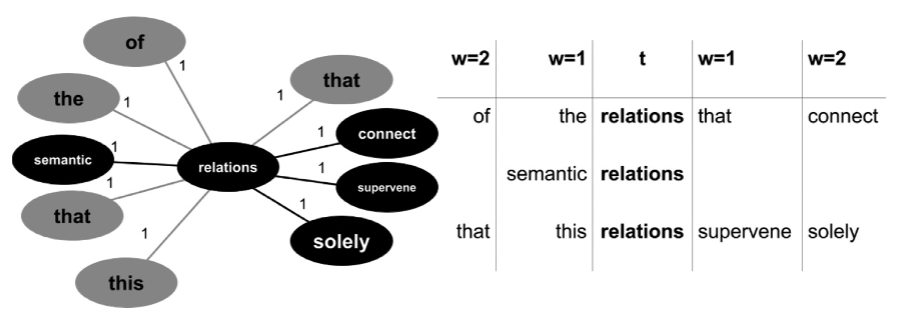
\includegraphics[width=0.7\linewidth]{src/img/coocurrences_example}
	\caption{Совместное появление при w = 2}
	\label{fig:coocurrencesexample}
\end{figure}

\begin{equation}
	DL[DR] = \frac{|A_t, w|}{\sum_{k \in A_{t, w}CoOccur_{t, k}}} 
\end{equation}
где $|A_t, w|$ представляет собой количество различных терминов, где термин представляет собой анализируемое содержимое, аббревиатуру, или слово в верхнем регистре, которое появляется слева(справа) от термина-кандидата t в заданном окне размера w \eqref{fig:coocurrencesexample} в отношении k терминов с которыми он встречается.

Затем DL и DR умножаются на частоту термина-кандидата, деленную на максимальную частоту термина среди всех кандидатов, которые встречаются в документе.
Окончательное уравнение имеет вид \eqref{eq:trel}:
\begin{equation}
	\label{eq:trel}
	T_{Rel} = 1 + (DL + DR) * \frac{TF_t}{MaxTF}
\end{equation}
где крайняя левая часть уравнения измеряет значимость термина-кандидата по отношению к его левой части, а
самая правая часть измеряет свою значимость по отношению к правой стороне. С практической точки зрения, чем менее релевантен кандидат t, тем выше будет оценка этой функции.
Таким образом, стоп-слова и, аналогичным образом, недискриминационные термины, как правило, получают более высокий балл. На рис. \eqref{fig:coocurrencesexample} показаны различные термины, которые встречаются вместе с термином-кандидатом «relations» в пределах w, равного 2, где «relations» — неважный термин (не часть истины, т. е. не золотое ключевое слово) в контексте нашего текущего примера.
В правой части рисунка показаны отрывки из текста, в которых встречается термин «отношения», а в левой — графическое представление. 
Число на ребрах — это частота, с которой термин-кандидат «relations» встречается вместе в соответствующем овале. 
Серым цветом обозначены стоп-слова.

\subsection{Другое предложение термина ($T_{sentence}$)}

Это свойство подсчитывает как часто термин-кандидат встречается в других предложениях.
Оно отображает, что кандидат, встречающийся во многих других предложениях, можеть быть более важным.
Оценка подчитывается по следующей формуле:

\begin{equation}
	T_{sentence} = \frac{SF(t)}{Sentences}
\end{equation}
где $SF(t)$ - количество предложений в которых появляется t.
$Sentences$ - это максимальное количесвто предолжений в тексте.
Результат лежит в диапозоне от $[0, 1]$


\subsection{Подсчет оценки термина}
После того как все оценки свойств получены, можно подсчитать финальный результат оценки термина.
Все полученные ранее оценки подставляются в выражение S(t) \eqref{eq:termin_score}.

\begin{equation}
	\label{eq:termin_score}
	S(t) = \frac{T_{Rel} * T_{Postion}}{T_{Case} + \frac{TF_{Norm}}{T_{Rel}} + \frac{T_{sentences}}{T_{Rel}}}
\end{equation}
Стоит обратить внимание на то что $TF_{Norm}$ и $TF_{sentensec}$ делятся на $T_{Rel}$.
Это делается для того чтобы присвоить большое значение терминам, которые появляются часто во многих предложениях, до тех пор пока они релевантны.
Поскольку, некоторые кандидаты могут встречаться много раз в многих предложениях и при этом быть бесполезными и должны быть "оштрафованы".
Таким образом достижение высокой оценки по $TF_{Norm}$ и $TF_{sentensec}$ является индикацией важности термина при низком значении $T_{Rel}$.
Так же важным свойством является позиция появления термина, она добавляется в выражение путем умножения $T_{Rel} * T_{Postion}$

\section{Сравнение методов}
\begin{enumerate}
	\item TF-IDF
	\item Плюсы \begin{enumerate}
		\item простой.
	\end{enumerate}
	\item Минусы \begin{enumerate}
		\item требует наличия большого корпуса текстов;
		\item не работает со словосочетаниями
		\item оценка происходит только по частотной характеристеке термина
	\end{enumerate}
	\item Rake
	\item Плюсы \begin{enumerate}
		\item простой
		\item не требует наличия корпуса текстов;
		\item учитывает взаимосвязи слов в тексте.
	\end{enumerate}
	\item Минусы \begin{enumerate}
		\item оценка происходит только по частотной характеристике термина
		\item не выдает словосочетания
	\end{enumerate}
	\item Yake
	\item Плюсы \begin{enumerate}
		\item учитывает взаимосвязи слов;
		\item учитывает позицию кандидата;
		\item учитывает его написание (абревиатуры, регистры);
		\item учитывается связь с контекстом
	\end{enumerate}
	\item Минусы \begin{enumerate}
		\item Не выдает словосочетания
	\end{enumerate}
\end{enumerate}

Учитывая все ранее выставленные требования к алгоритмам было принято решение использовать метод Yake.
До этого данный метод не использовался для вычисления ключевых слов из текста на русском языке и для этого необходимо провести следующие модификации:
\begin{enumerate}
	\item добавление сборника стоп-слов;
	\item добавление работы с N-gram;
\end{enumerate}

\section{Модификация}
Шумовые слова (или стоп-слова) — термин из теории поиска информации по ключевым словам.
Это такие слова, знаки, символы, которые самостоятельно не несут никакой смысловой нагрузки, но
которые, тем не менее, совершенно необходимы для нормального восприятия текста, его целостности.
К ним относятся предлоги, суффиксы, причастия, междометия, цифры, частицы и т. п.
Так как данные слова имеют самые большие частоты встречи в документах, то для более корректного результата небходимо данные слова исключать из текста, по этому есть необходимость в добавлении в метод списка стоп-слов для русского языка.

Как было описано ранее, результатом работы метода Yake являются одиночные ключевые слова с оценкой.
Современные технологии непрерывно развиваются.
Это значительно влияет на научно-технический функциональный стиль, в частности, на его терминосистемы.
Появляются новые термины и усложняются старые \cite{22}.
В результате растет количество многокомпонентных терминов.
По этому есть необходимость в модификации выбранного метода для возможности извлечения многокомпонентных ключевых слов.
Данную модификацию проведем с помощью добавления n-грамм.
Пусть задан некоторый конечный алфавит $V = {w_i}$, где $w_i$ - символ. 
Языком $L(V)$ называют множество цепочек конечной длины из символов $w_i$.
Высказыванием называют цепочку из языка.
N-граммой на алфавите V называют произвольную цепочку длинной N, например последовательность из N букв русского языка, одного слова, одной фразы, одного текста \cite{21}.

Конечный результат будет высчитываться по формуле \eqref{eq:ngram}: 
\begin{equation}
	\label{eq:ngram}
	S(kw) = \frac{\prod_{t \in kw}S(t)}{KF(kw) * (1 + \sum_{t \in kw}S(t))}
\end{equation}
где $S(kw)$ - финальный результат оценки, чем ниже тем реливантнее, $S(t)$ - оценка одиночного термина,
$KF(kw)$ - частота ключевого слова(выражения)

\section{Заключение}
В рамках данного раздела представлено описание предметной области задачи по извлечению ключевых слов. 
Приведена систематизация методов извлечения КС и текстов.
Произведен отбор и сравнение методов удовлетворяющих выставленным ограничениям.
Отобран метод на базе которого будет проводиться модификация
Определены направления модификации выбранного метода Yake.



\chapter{Конструкторский раздел}
В данном разделе приведено описание структуры алгоритма и отдельных его этапов с помощью диаграммы IDEF0.
Продемонстрирована схема этапа предварительной обработки текста.
Представлена архитектура и выставлены требования к пользовательскому интерфейсу разрабатываемого программного обеспечения
Продемонстрирована диаграмма классов, использующихся в работе

\section{Yake}
Общая структура метода извлечения ключевых слов представлена на рисунках \ref{fig:01a0} - \ref{fig:02a0}
\begin{figure}[!h]
	\centering
	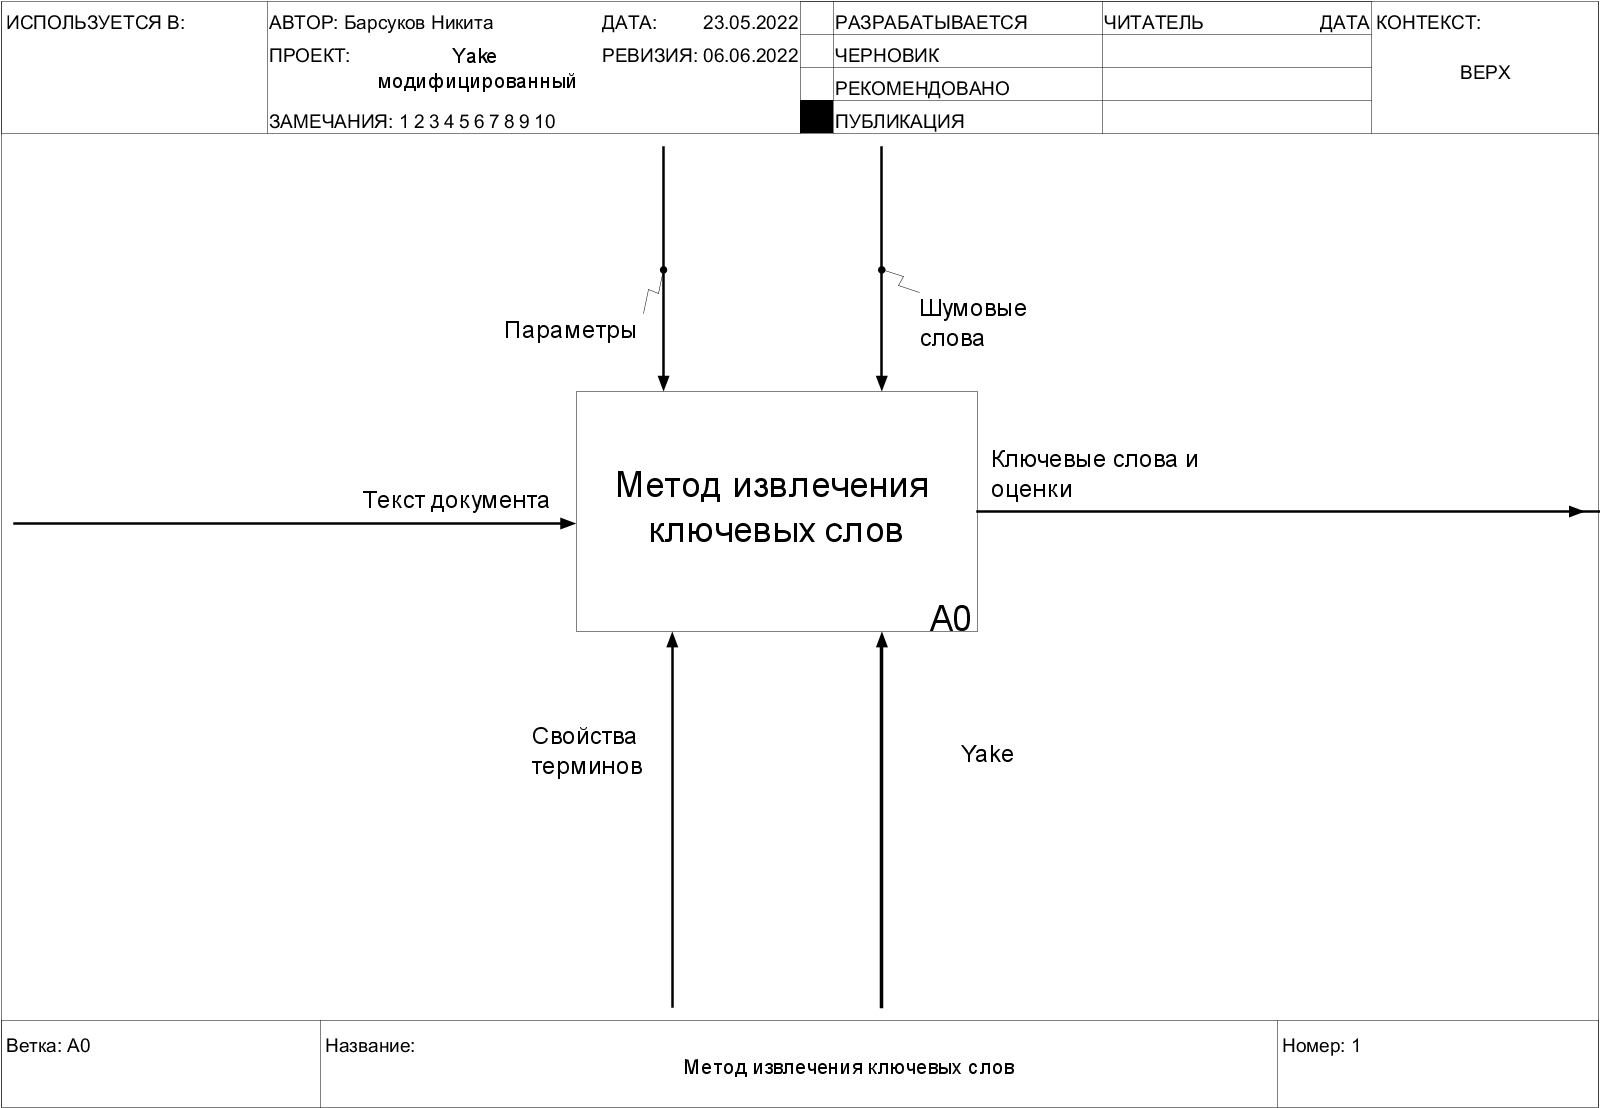
\includegraphics[width=1\linewidth]{src/img/idef0/Yake/01_A0}
	\caption{IDEF0 диаграмма разрабатываемого метода}
	\label{fig:01a0}
\end{figure}
Входными параметрами данного алгоритма являются тест извлеченный из электронного документа и язык работы.
Результатом исполнения данного метода является список, состоящий из кортежей, содержащих в себе термин и его оценку.

Данный метод можно разделить на несколько основных этапов, которые представлены на IDEF0-диаграмме, изображенной на рисунке \ref{fig:02a0}
\begin{figure}[!h]
	\centering
	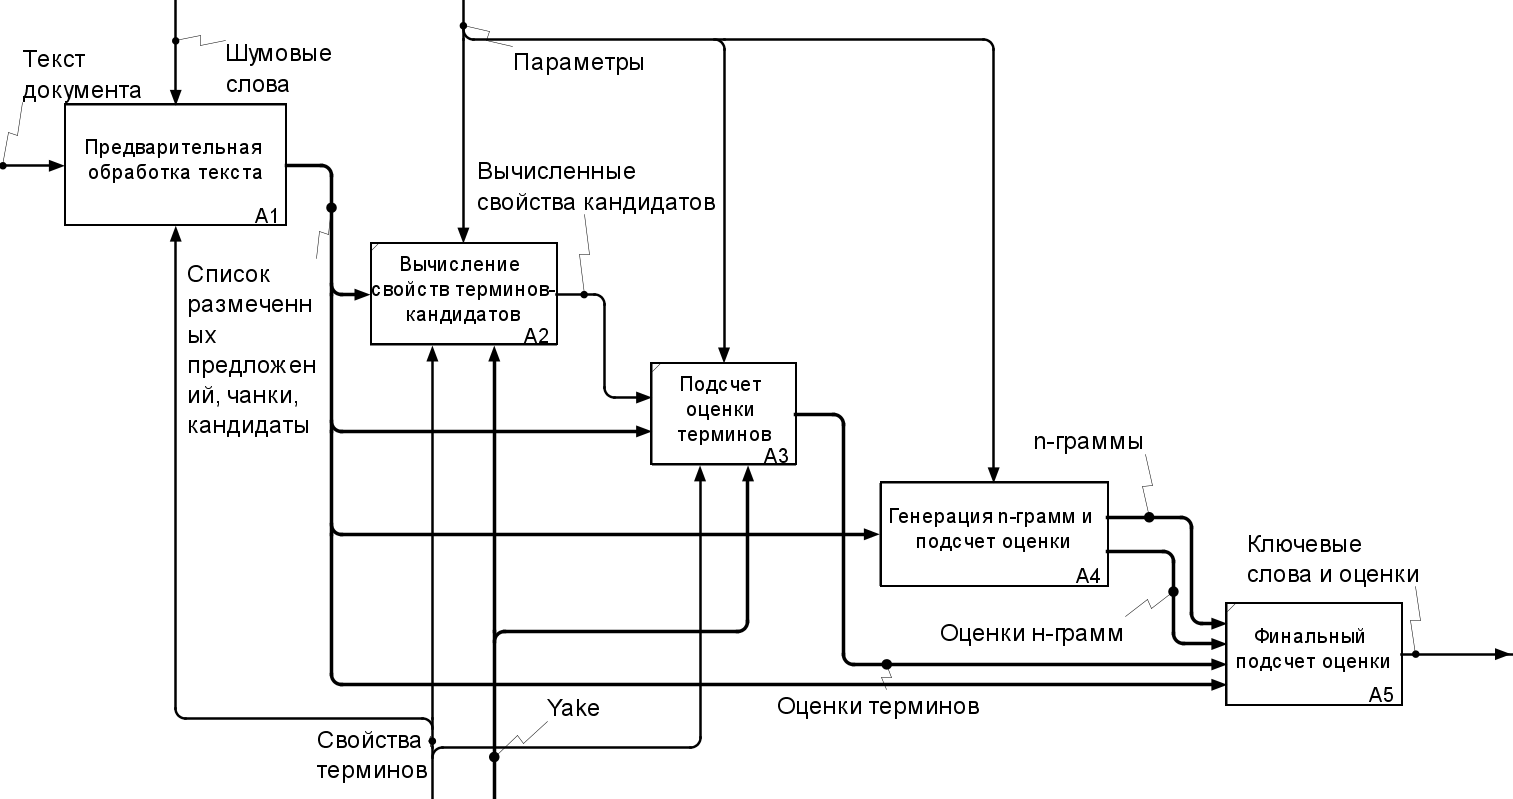
\includegraphics[width=1\linewidth]{src/img/idef0/Yake/02_A0}
	\caption{IDEF0 диаграмма модуля извлечения ключевых слов из текста}
	\label{fig:02a0}
\end{figure}

\begin{enumerate}
	\item предварительная обработка текста и выделение кандидатов (рисунок \ref{fig:02a0} блок А1)
	\item вычисление свойств термин-кандидатов (рисунок \ref{fig:02a0} блок А2)
	\item подсчет оценки кадидатов (рисунок \ref{fig:02a0} блок А3)
	\item генерация н-грамм и подсчет оценки (рисунок \ref{fig:02a0} блок А4)
	\item подсчет финальной оценки терминов (рисунок \ref{fig:02a0} блок А5)
\end{enumerate}

Формально этап обработки и выделения кандидатов, отображен на рисунке \ref{fig:03a1}
\begin{figure}[!h]
	\centering
	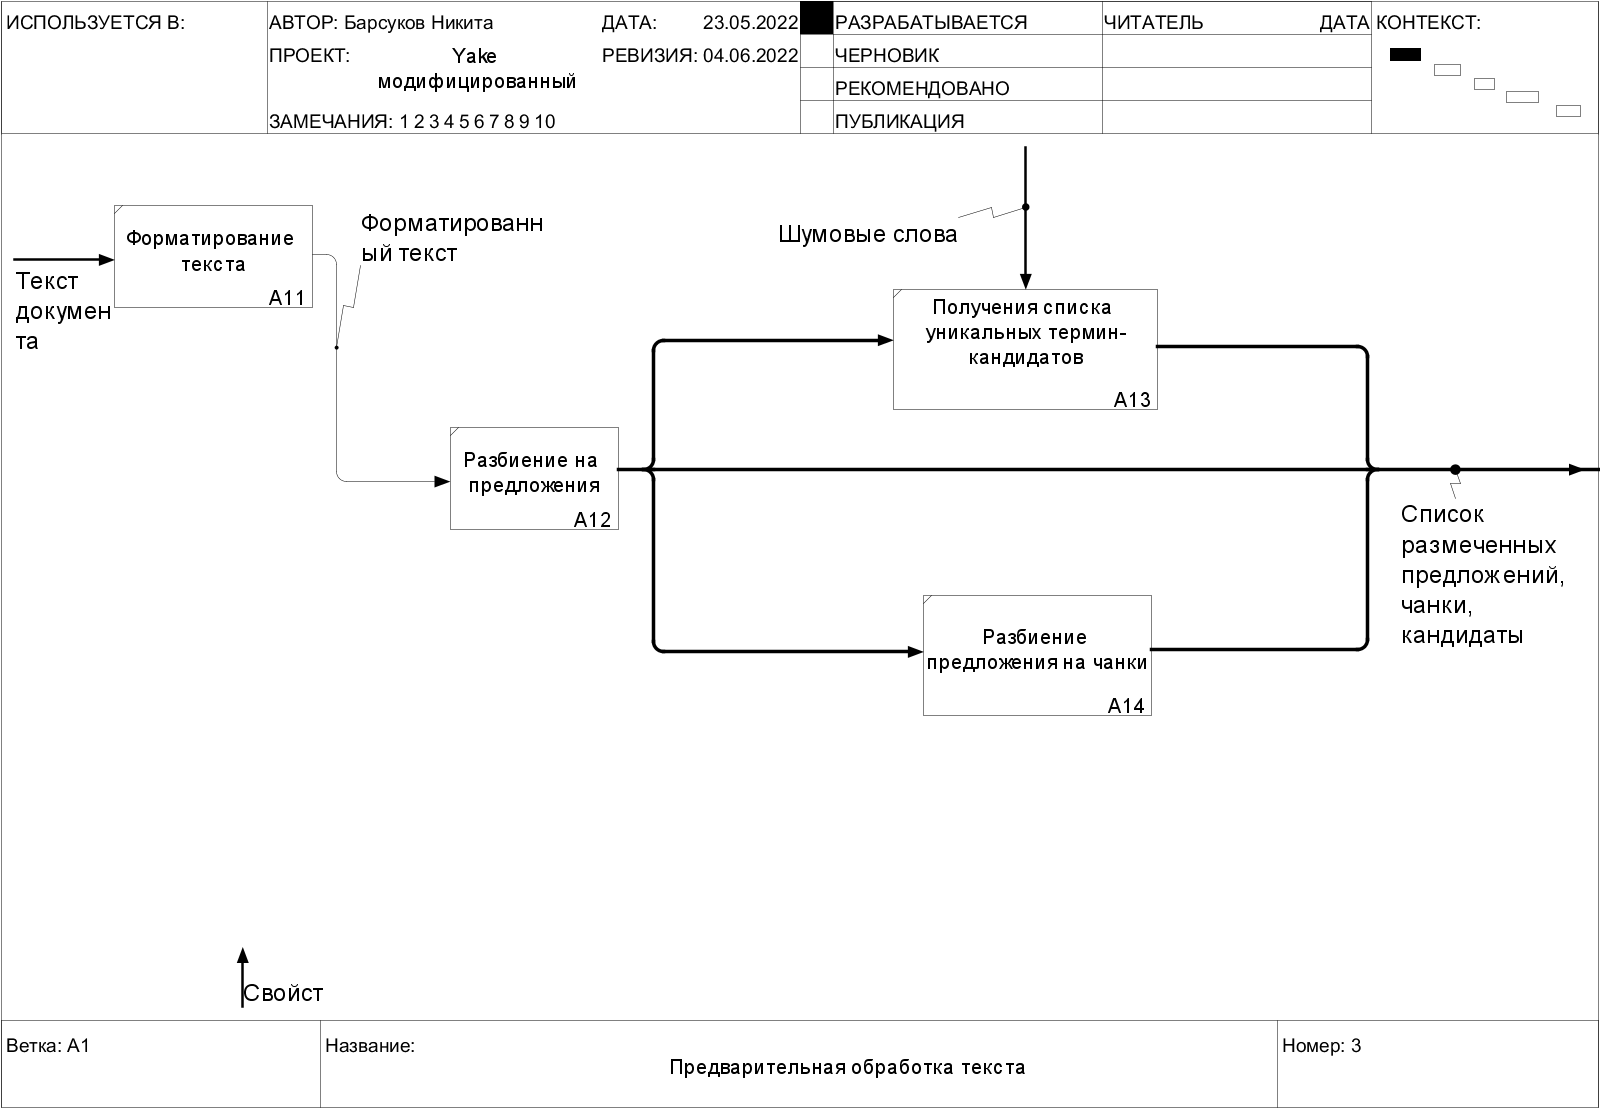
\includegraphics[width=1\linewidth]{src/img/idef0/Yake/03_A1}
	\caption{IDEF0 диаграмма этапа предварительного этапа обработки текста}
	\label{fig:03a1}
\end{figure}

\begin{figure}[!h]
	\centering
	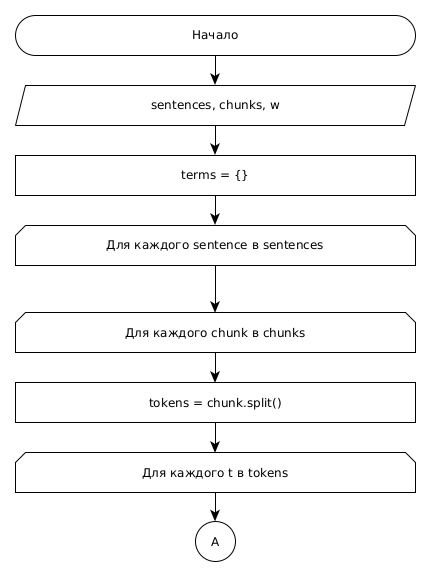
\includegraphics[width=0.7\linewidth]{src/img/design/feature_ext_1}
	\caption{Начало извлечения характеристик}
	\label{fig:featureext1}
\end{figure}

\begin{figure}[!h]
	\centering
	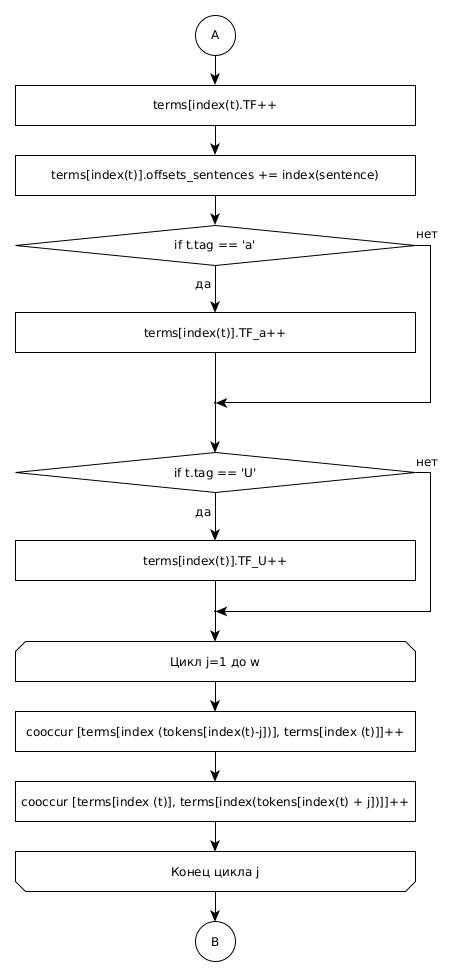
\includegraphics[width=0.6\linewidth]{src/img/design/feature_ext_2}
	\caption{Извлечение характеристик}
	\label{fig:featureext2}
\end{figure}

\begin{figure}[!h]
	\centering
	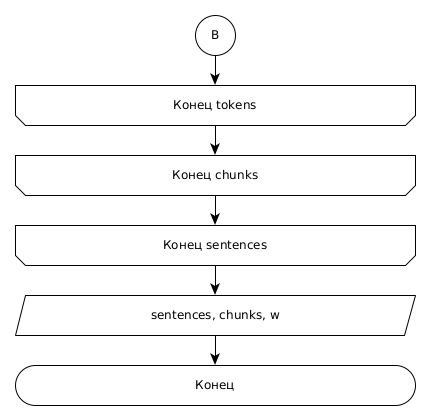
\includegraphics[width=0.7\linewidth]{src/img/design/feature_ext_3}
	\caption{Завершение извлечения характеристик}
	\label{fig:featureext3}
\end{figure}
В начале происходит предварительное форматирование текста, путем замены спецсимволов, таких как табуляция, перенос на новую строку и т.п. на пробелы.
Затем текст разбивается на предложения, а сами предложения на сегменты, используются на этапе оценки свойств кандидатов и построении н-грамм. 
После этого из полученных данных извлекаются уникальные термин-кандидаты с контекстной информацией.

Для оценки валидности терминов необходимо вычислить их статистические свойства и характеристики.
На рисунках \ref{fig:featureext1}, \ref{fig:featureext2} и \ref{fig:featureext3} отображена схема вычисления характеристик, где $TF$ - частота термина, $TF\_U$ - частота термина в верхнем регистре, $TF\_a$ - частота термина в виде аббревиатуры.
Теперь необходимо вычислить свойства терминов, процесс вычисления отображен на рисунках \ref{fig:calculate1}
\begin{figure}[!h]
	\centering
	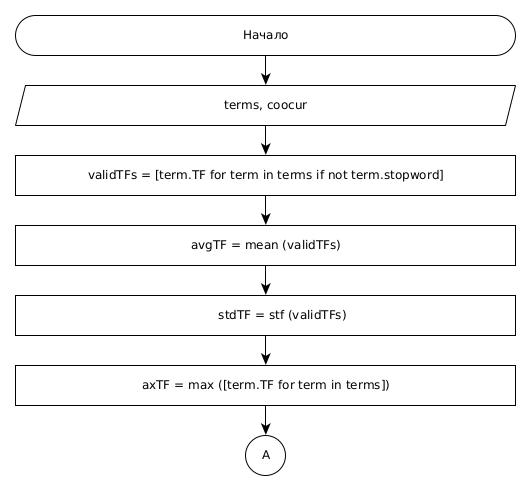
\includegraphics[width=0.7\linewidth]{src/img/design/calculate_1}
	\caption{Вычисление общих свойств}
	\label{fig:calculate1}
\end{figure}

\begin{figure}[!h]
	\centering
	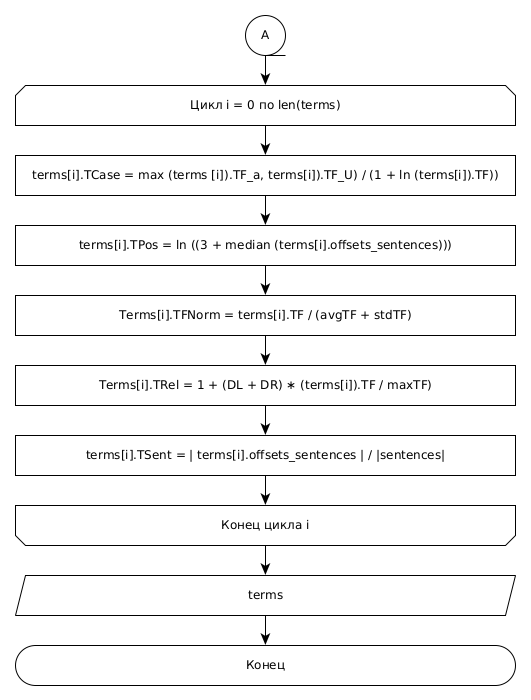
\includegraphics[width=0.7\linewidth]{src/img/design/calculate_2}
	\caption{Вычисление свойств для каждого термина}
	\label{fig:calculate2}
\end{figure}

После получениях всех свойств для каждого термина идет процесс выбора н-грамм и подсчет оценки.
Так оценка н-грамм строится на основе оценок одиночных терминов, то остается только объединить результаты и отсортировать полученный список по релевантности.


\section{Архитектура ПО}
Для реализации программного обеспечения была выбрана MVC (Model-View-Controller) архитектура, разбивающая программу на три отдельных компонента:
\begin{enumerate}
	\item представление - это отображение состояния внутренней системы;
	\item модель - это компонента, отвечающая за предоставление данных конкретным элементам системы;
	\item контроллер - это связующее звено между представлением и моделью, обрабатывает действия пользователя, полученные от представления и отдает команды модели.
\end{enumerate}
\begin{figure}[!h]
	\centering
	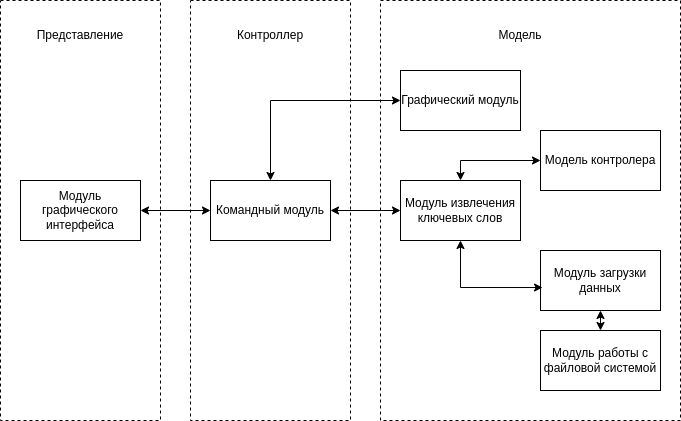
\includegraphics[width=1\linewidth]{src/img/design/mvc.drawio}
	\caption{Схематичное преставление архитектуры ПО}
	\label{fig:mvc}
\end{figure}

Благодаря использованию MVC подхода к организации архитектуры ПО, воздействие в случаи модификации или замены модуля на другие компоненты сводится к минимуму или полностью отсутствует, что добавляет системе гибкости.
Это достигается путем разделения: работы с данными, логики взаимодействия пользователя с интерфейсом.
Отличительной чертой данного решения является принцип чистой архитектуры, основанный на разделении данных.
Каждый компонент системы должен легко и просто заменяться другим и на оборот.
Это же касается используемых инструментов, библиотек, фрейворков, то есть система не привязана к конкретным технологиям и их в любой момент можно заменить.

Через графический интерфейс у пользователю должна быть возможность взаимодействия с программный ПО. 
Под взаимодействием подразумевается запуск ПО и получения результата.
Предоставляющийся функционал:
\begin{enumerate}
	\item выбор из списка методов извлечения КС от одного до нескольких алгоритмов;
	\item выбор одного или нескольких файлов через специальное окно;
	\item установка параметров для методов в отдельном окне;
	\item возможность ввести отдельно текстовую информацию.
\end{enumerate}

На рисунке \ref{fig:classdiagram} схематично отображены основные классы разрабатываемого программного продукта

Класс MainWindow - это входная точка приложения.
Он выполняет основную логику, связанную с обработкой пользовательский запросов к графическому интерфейсу.
Он взаимодействует с классом MethodControler, отвечающим за подгрузку, подготовку методов к работе и запуск процесса извлечения ключевых слов. Сами методы представлены в виде классов.

\begin{figure}[!h]
	\centering
	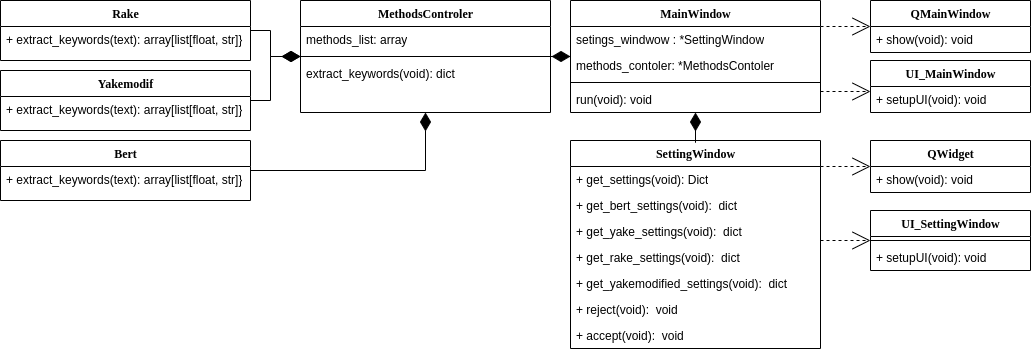
\includegraphics[width=1\linewidth]{src/img/class_diagram}
	\caption{Схематическое представление архитектуры классов программного обеспечения}
	\label{fig:classdiagram}
\end{figure}

\section{Вывод}
В данном разделе было спроектировано программное обеспечение для извлечения ключевых слов и словосочетаний из электронного документа на русском языке. 
Представлены диаграммы IDEF0 и описаны основные компоненты ПО.
Результаты проектирования:
\begin{enumerate}
	\item спроектирована архитектура разрабатываемого ПО;
	\item модификация алгоритма путем применения н-грамм;
	\item разработана структура ПО.
\end{enumerate}



\chapter{Технологический раздел}
В разделе проведен обзор актуальных языков программирования на основе которого был выбран ЯП для реализации разрабатываемого программного обеспечения.
Приведено описание используемых библиотек и фреймворков.
Приведено описание входных и выходных данных. 
Продемонстрирована работа ПО на рисунках \ref{fig:nbarsukov20220605a9ea}, \ref{fig:settings}
Обоснован выбор интегрированной среды разработки IDE и системы контроля версий VCS

\section{Системные требования}
Каждое программное обеспечение требует материальной базы, в рамках которой оно будет функционировать.
Описание характеристик такой базы, называется системными требованиями.
Данные требования предоставляют пользователю информацию об аппаратном обеспечении, необходимом для использования ПО.
\begin{enumerate}
	\item Операционная система: Ubuntu 18.04.6 TLS
	\item Процессор: Intel(R) Core(TM) i5-8265U CPU @ 1.60GH	3900,00 MHz	
	\item Жесткий диск: 500 гб
	\item Оперативная память: 16гб
\end{enumerate}

\section{Язык программирования}
Продолжающееся развитие компьютерных технологий и широкое их распространие, спровоцировало спрос на развитие и создание новых знаковых систем для записи алгоритмов, которые известны на сегодняшний день как языки программирования (ЯП).
Сформируем список из наиболее популярных и проведем обзор для установления их соответствия поставленной задаче.
\begin{enumerate}
	\item Python;
	\item C++;
	\item C\#;
\end{enumerate}

В данный список не попали языки, относящиеся к веб-разработке, поскольку разрабатываемое программное обеспечение представляет собой декстопное приложение.

\subsection{Python}
Python –  это высокоуровневый язык программирования общего назначения, который ориентирован на повышение читаемости кода и удобства использования разработчиком. 
ЯР Python минималистичен. 
В то же время стандартная библиотека содержит в себе разнообразный набор полезных, в ходе разработки, функций.

Python поддерживает несколько парадигм программирования, в том числе:
\begin{enumerate}
	\item структурное;
	\item объектно-ориентированное;
	\item императивное;
	\item аспектно-ориентированное;
	\item функциональное.
\end{enumerate}
Основными архитектурными чертами, являются такие особенности, как автоматическое управление памятью, динамическая типизация, механизм обработки исключений, полная интроспекция, гибкие высокоуровневые структуры данных и поддержка многопоточных вычислений. 
Код в Python организовывается в классы и функции, которые могут объединяться в модули, которые, в свою очередь, могут быть объединены в пакеты. 

Эталонной реализацией Python является интерпретатор CPython, поддерживающий большинство активно используемых платформ. Он распространяется под свободной лицензией Python Software Foundation License, которая
позволяет использовать его без ограничений в любых приложениях, включая проприетарные. 
Наиболее часто Python сравнивают с Ruby и Perl. Эти языки обладают примерно одинаковой скоростью выполнения программ и также являются интерпретируемыми.

\subsection{C++}
С++ - это универсальный язык программирования. 
За исключением второстепенных деталей С++ является надмножеством языка программирования С. 
Помимо возможностей, которые дает С, С++ предоставляет эффективные и гибкие средства определения новых типов. Используя определения новых типов, точно отвечающих концепциям приложения, программист может разделять разрабатываемую программу на легко поддающиеся контролю части. 
Такой метод построения программ часто называют абстракцией данных.
Информация о типах содержится в некоторых объектах типов, определённых пользователем. 
Такие объекты просты и надёжны в использовании, в тех ситуациях, когда их тип нельзя установить на стадии компиляции.

Программирование с применением таких объектов часто называют объектно-ориентированным. 
При правильном использовании этот метод даёт легче контролируемые программы, более короткие и проще понимаемые. 
С++ предлагает программисту полный набор операторов структурного программирования. Он также обладает очень большим набором операций. 
Многие операции С++ соответствуют машинным командам, и поэтому допускают прямую трансляцию в код ассемблера. Разнообразие, предоставляемое С++ позволяет выбирать их различные наборы для минимизации результирующего поля. 
С++ поддерживает указатели на переменные и функции. 
Указатель на объект программы соответствует машинному адресу данного объекта. 
Посредством разумного использования указателей можно создавать эффективные программы, которые выполняются быстро, так как указатели позволяют ссылаться на объекты тем же самым путём, как это делает машина.

\subsection{C\#}
C\# – это объектно-ориентированный язык программирования. Разработан в 1998-2001 годах в компании Microsoft в качестве языка разработки приложений для платформы Microsoft .NET Framework и впоследствии был стандартизирован как ISO/IEC 23270 и ECMA-334. C\# относится к семье языков с C-подобным синтаксисом, среди них его синтаксис наиболее близок к C++ и Java. 
Язык поддерживает полиморфизм, перегрузку операторов (в том числе операторов неявного и явного приведения типа), имеет статическую типизацию, атрибуты, делегаты, свойства, события, обобщённые методы и типы, анонимные функции с поддержкой замыканий, итераторы, LINQ-запросы,
комментарии в формате XML и исключения.

В результате сравнения языков программирования оптимальным является Python.
Python будет использоваться для модулей логики и взаимодействия.
Установление связи между компонентами будет обеспечено с помощью применения слотов и сигналов из библиотеки PyQt5.

\section{Формат входных данных}
На вход программы ожидается файл формата PDF, содержащий в себе текст, написанный на русском языке, длинной не меньше 50 слов, относящийся к одной теме (статье). Для хранения файлов используется файловая система.

Формат переносимых документов (PDF) представляет собой универсальный тип файлов, который позволяет сохранить шрифты, изображения и сам макет исходного документа, независимо от того, на какой из множества платформ и в каком из множества приложений такой документ создавался. 
Формат Adobe PDF считается признанным общемировым стандартом в области тиражирования и обмена надежно защищенными электронными документами и бланками \cite{23}

\section{Библиотеки}
Современное программное обеспечение состоит из множества компонентов. 
Полная реализация всех необходимых модулей самостоятельно, увеличивала бы и без того продолжительный процесс разработки.
Для решения данной проблемы используются библиотеки и фреймворки, которые предоставляют часть или полностью готовый функционал.
Для реализации данной работы использовались следующие библиотеки:
\begin{enumerate}
	\item numpy;
	\item networkx;
	\item segtok;
	\item jellyfish;
	\item poetry;
	\item textract;
\end{enumerate}
\textit{NumPy} - это фундаментальный пакет для научных вычислений в Python. 
Который предоставляет многомерный объект массива, различные производные объекты (такие как маскированные массивы и матрицы) и ассортимент подпрограмм для быстрой работы на массивах, в том числе манипулирование формой, сортировка, выбор, дискретные преобразования Фурье, базовая линейная алгебра, основные статистические операции, случайное моделирование и многое другое.

\textit{jellyfish} -  представляет из себя набор функций для стемминга (процесса нахождения начальной формы слов), реализаций методов нахождения редакционного расстояния таких как: расстояние Левенштейна, Дамерау-Левенштейна, Хамминга и Жаро.

\textit{Segtok} - библиотека содержащая две модели segmenter и tokenizer. Segmenter предоставляет функционал по разделению текста Индо-Европейских языков на предложения.
Tokenizer предоставляет инструмент для разбиения предложений на слова и символы.

\textit{Networkx} - это библиотека для теории графов и средство моделирования сети, разработанное на языке Python, которое содержит встроенные графы и сложные алгоритмы сетевого анализа.
Networkx, позволяет хранить сети в стандартизированных и нестандартизированных форматах данных, анализировать сетевые структуры, создавать модели сетей, разрабатывать новые сетевые алгоритмы и выполнять рендеринг сети.
Networkx поддерживает создание простых ориентированных, неориентированных и мульти-графов; во многих стандартных алгоритмах теории графов узлами могут быть любые данные; поддерживается любое измерение граничных значений.
Прост в использовании.
В рамках работы, используется для определения совместного появления терминов, на этапе оценки свойств методов.

\textit{Poetry} - это инструмент для управления зависимостями и сборкой пакетов в Python.
В Poetry представлен полный набор инструментов, которые могут понадобиться для детерминированного управления проектами на Python. В том числе сборка пакетов, поддержка разных версий языка, тестирование и развертывание проектов.

\section{Графический интерфейс}
Для реализации пользовательского интерфейса была выбрана библиотека PyQt5, которая предоставляет возможность создавать графические интерфейсы для пользователя. 
Она предоставляет объектно-ориентированные решения, которые включают в себя логическую иерархию между объектами, имеет понятную структуру наследования.
Данное пакетное решение является бесплатным, распространяется по лицензии GPL, LGPL.
Для проектирования интерфейса использовался QtDesigner.
Данный программное обеспечение  входит в набор разработчика QT.
Служит для разметки интерфейса в формате XML.
Формат преобразуется в питоновский класс интерфейса с помощью специального парсера pyuic5.

На рисунках \ref{fig:nbarsukov20220605a9ea} - \ref{fig:nbarsukov202206056adf} представлен интерфейс разрабатываемого ПО.

% TODO: \usepackage{graphicx} required
\begin{figure}[!h]
	\centering
	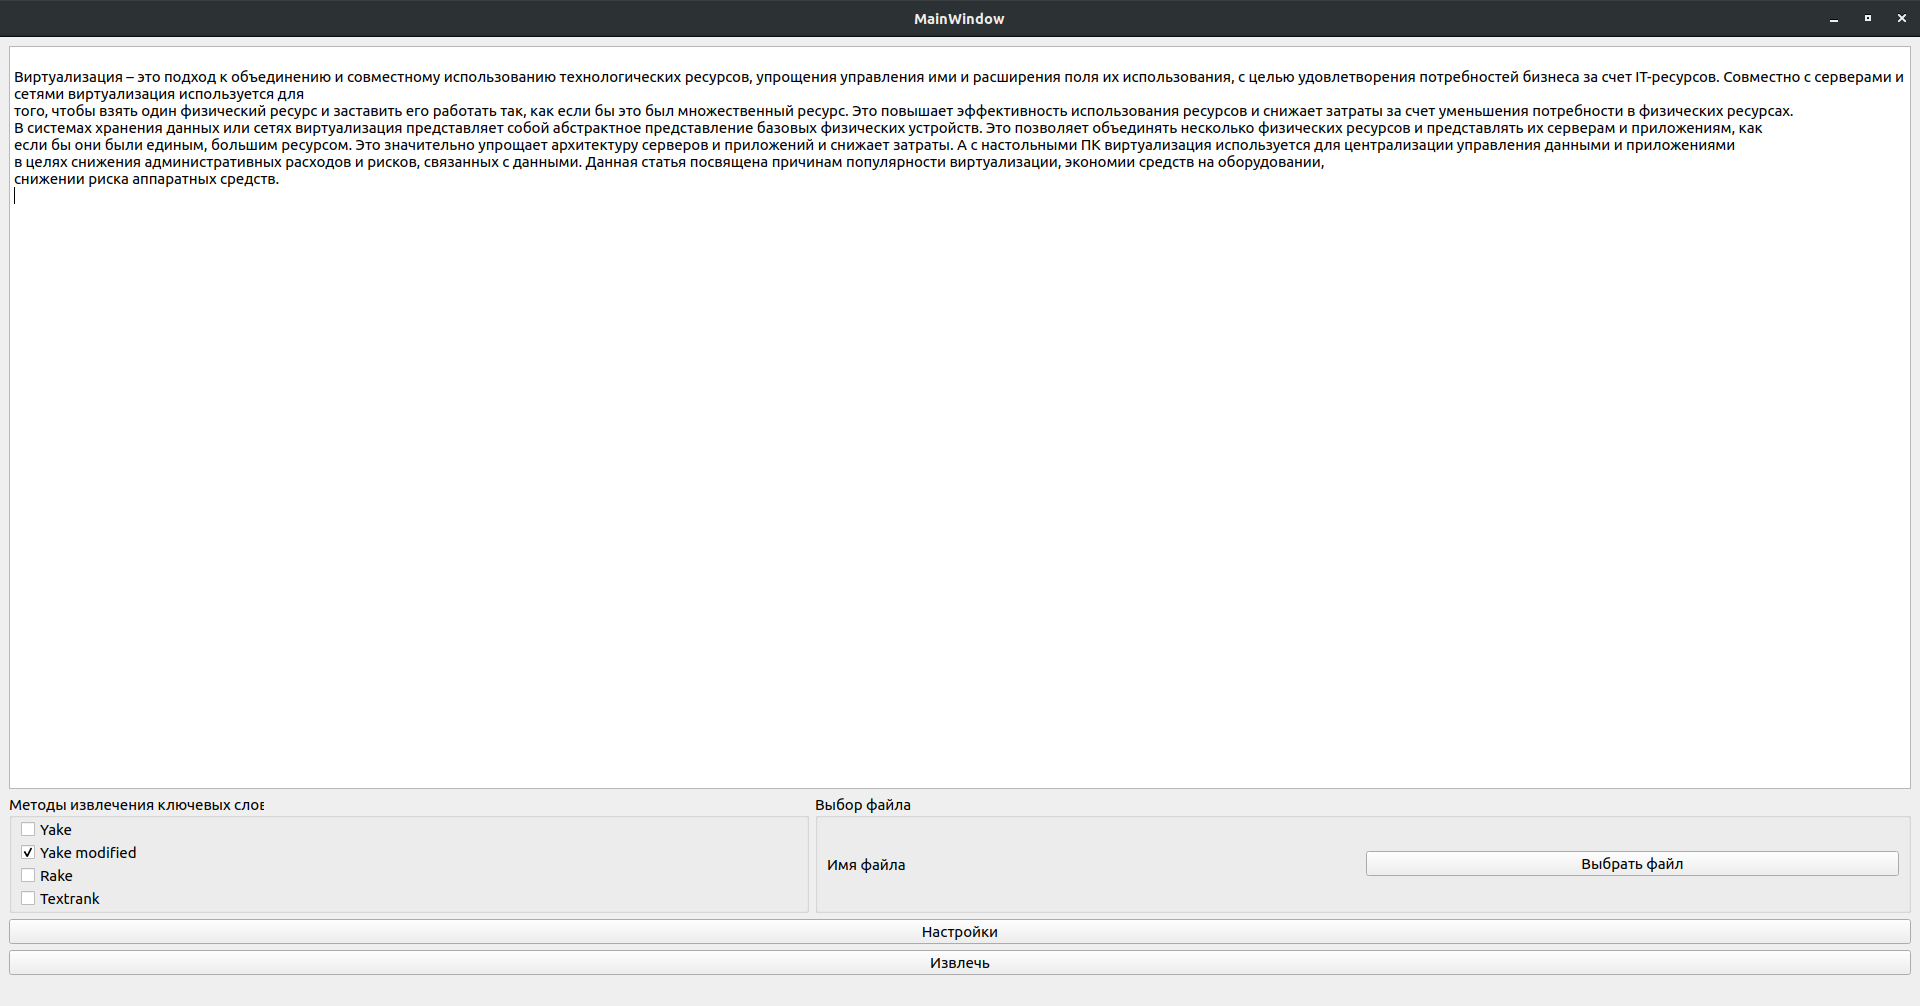
\includegraphics[width=0.7\linewidth]{src/img/tech/nbarsukov_20220605_a9ea}
	\caption{Главное окно}
	\label{fig:nbarsukov20220605a9ea}
\end{figure}


\begin{figure}[!h]
	\centering
	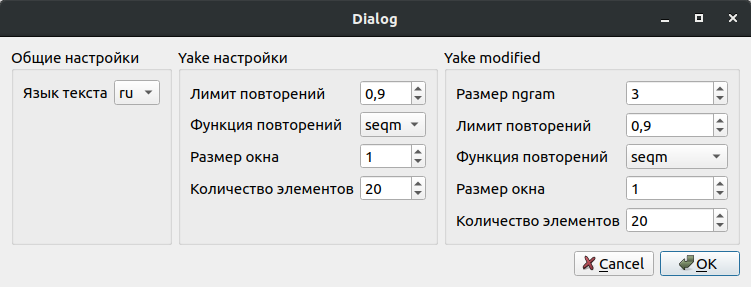
\includegraphics[width=0.7\linewidth]{src/img/programm/settings}
	\caption{Окно настроек методов}
	\label{fig:settings}
\end{figure}

% TODO: \usepackage{graphicx} required
\begin{figure}
	\centering
	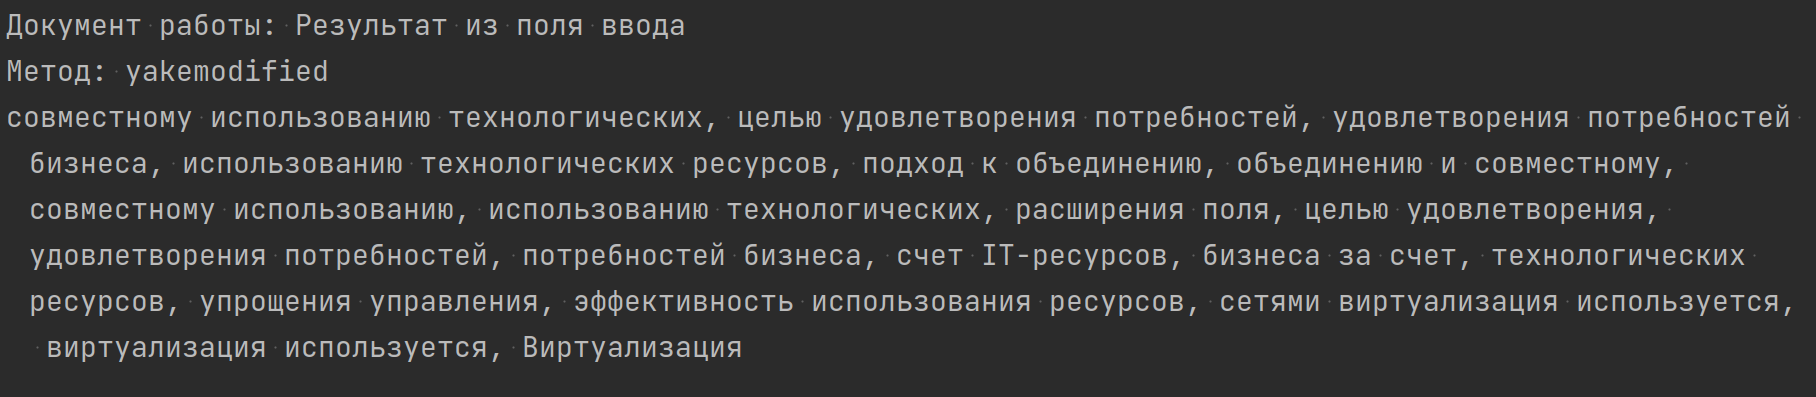
\includegraphics[width=0.7\linewidth]{src/img/tech/nbarsukov_20220605_6adf}
	\caption{Результат извлечения ключевых слов}
	\label{fig:nbarsukov202206056adf}
\end{figure}

Пользовательский интерфейс состоит из нескольких окон.
На рисунке \ref{fig:nbarsukov20220605a9ea} представлено главное окно программы.
В данном окне пользователь может указать фрагмент текста, выбрать файл формата pdf для дальнейшего извлечение текстовой информации, выбрать алгоритмы, открыть окно c параметрами методов, изображенное на рисунке \ref{fig:settings} и запустить процесс извлечения ключевых слов.

На вход ожидаются:
\begin{enumerate}
	\item параметры методов;
	\item документ формата pdf или тест
\end{enumerate}
На выходе получем список кортежей, состоящий из ключевых слов и оценок.
Результат работы алгоритма, отображен на рисунке \ref{fig:result} и представляет собой список извлеченных ключевых слов.

\section{Среда разработки}
Интегрированная среда разработки или IDE (Integrated Development Environment) - специальный программный комплекс, предназначенный для полного цикла написания и тестирования программ на определенном языке.

Интегрированная среда разработки облегчает работу, предоставляя программистам средства для разработки программного обеспечения, такие как редактор исходного кода, средства автоматизации сборки и отладчик. 
IDE облегчает визуальное представление файлов и делает его более понятным для пользователя.

Средой разработки для разработки ПО была выбрана IDE PyCharm от компании JetBrains, специализирующейся на производстве инструментов для профессиональной разработки программного обеспечения.
Данная среда была выбрана из за следующих удобств и преимуществ:
\begin{enumerate}
	\item наличие полноценного отладчика как для кода так и для тестов;
	\item встроенная подсветка синтаксиса;
	\item встроенный терминал;
	\item интеграция с системой контроля версий (VCS) git;
	\item поддержка множественных конфигураций запуска;
	\item встроенный анализатор классов;
\end{enumerate}

\section{Система контроля версий}
Во время процесса разработки мною была использованна система контроля версий Git (https://git-scm.com). 
Система контроля версий с помощью репозиториев решает проблемы с переносом программного кода на другие устройства, его резервным копированием, а так же дает возможность разделения версий продукта во время разработки, что позволяет при внесении изменений или модификациях всегда иметь рабочею версию проекта.

\section{Вывод}
В результате выполнения данного раздела был выбран язык программирования и инструменты в виде библиотек и фреймворков, необходимых для реализации разрабатываемого программного обеспечения.
Проведен детальной обзор разработанного пользовательского интерфейса с применением QT5.
Описаны входные и выходные данные разрабатываемого метода.
Обоснован выбор интегрированной среды разработки IDE и системы контроля версий VCS

\chapter{Исследовательский раздел}
В данном разделе произведен ряд экспериментов с полученным, в ходе написания проекта, программным обеспечением.
Для проведения серии экспериментов необходимо подготовить набор тестовых входных данных, представляющих собой тридцать электронных документов на русском языке, формата PDF.
Все работы участвующие в эксперименте взяты с сайта \href{https://cyberleninka.ru/article}{cyberleninka.ru}
Для тестов отбираются тексты с указанными ключевыми словами.
Для удобства анализа, многокомпонентные ключевые слова из документов разбиваются на отдельные термины.

Для обеспечения качества проводимых экспериментов необходимо указать критерии по которым будет производиться отбор документов:
\begin{enumerate}
	\item документ должен содержать в себе текст, а не отсканированные изображения страниц ранее опубликованных работ, поскольку это приводит к невозможности прочтения документа;
	\item информация, содержащаяся в документе должна быть целостной, то есть принадлежать одной работе.
\end{enumerate}

\section{Исследование характеристик метода}
В процессе данного эксперимента ставится задача сравнить модифицированный метод с аналогами, способными на работу с документами на русском языке.
Для этой цели были выбраны следующие алгоритмы:
\begin{enumerate}
	\item Rake;
	\item Textrank.
\end{enumerate}
В качестве тестовых данных использовались тридцать ранее отобранных документов с ключевыми словами.
Исследуется процент от ключевых слов полученных из метода, попавших в пересечение с словами выделенными авторами, так же изучется процент не попавших в пересечение

Для методов были выбраны следующие настройки, отображенные на рисунке \ref{fig:nbarsukov20220605a9e9}
% TODO: \usepackage{graphicx} required
\begin{figure}[!h]
	\centering
	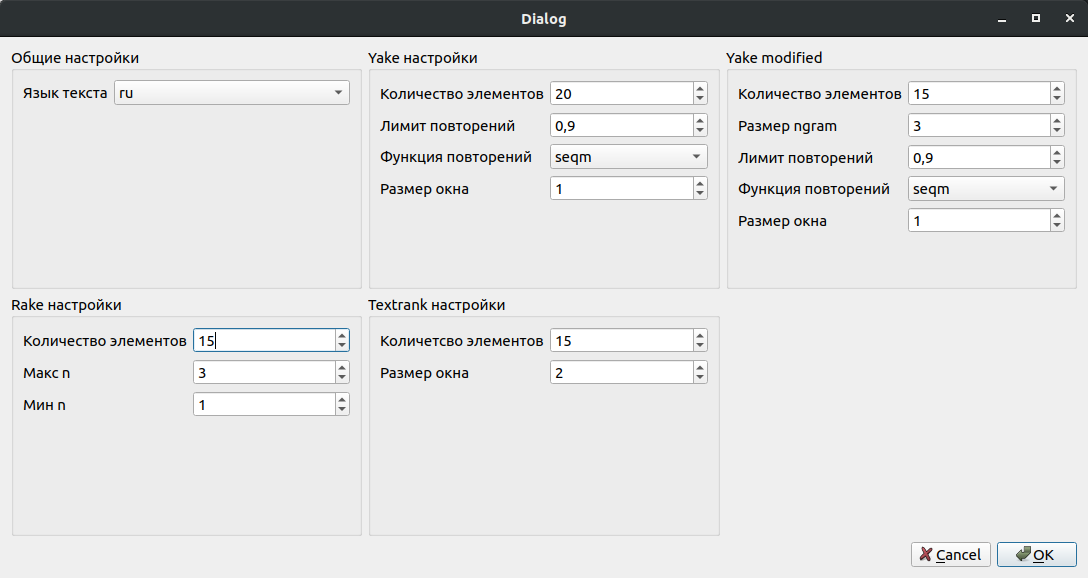
\includegraphics[width=0.7\linewidth]{src/img/experiment/nbarsukov_20220605_a9e9}
	\caption{Настройки методов}
	\label{fig:nbarsukov20220605a9e9}
\end{figure}

% TODO: \usepackage{graphicx} required
\begin{figure}
	\centering
	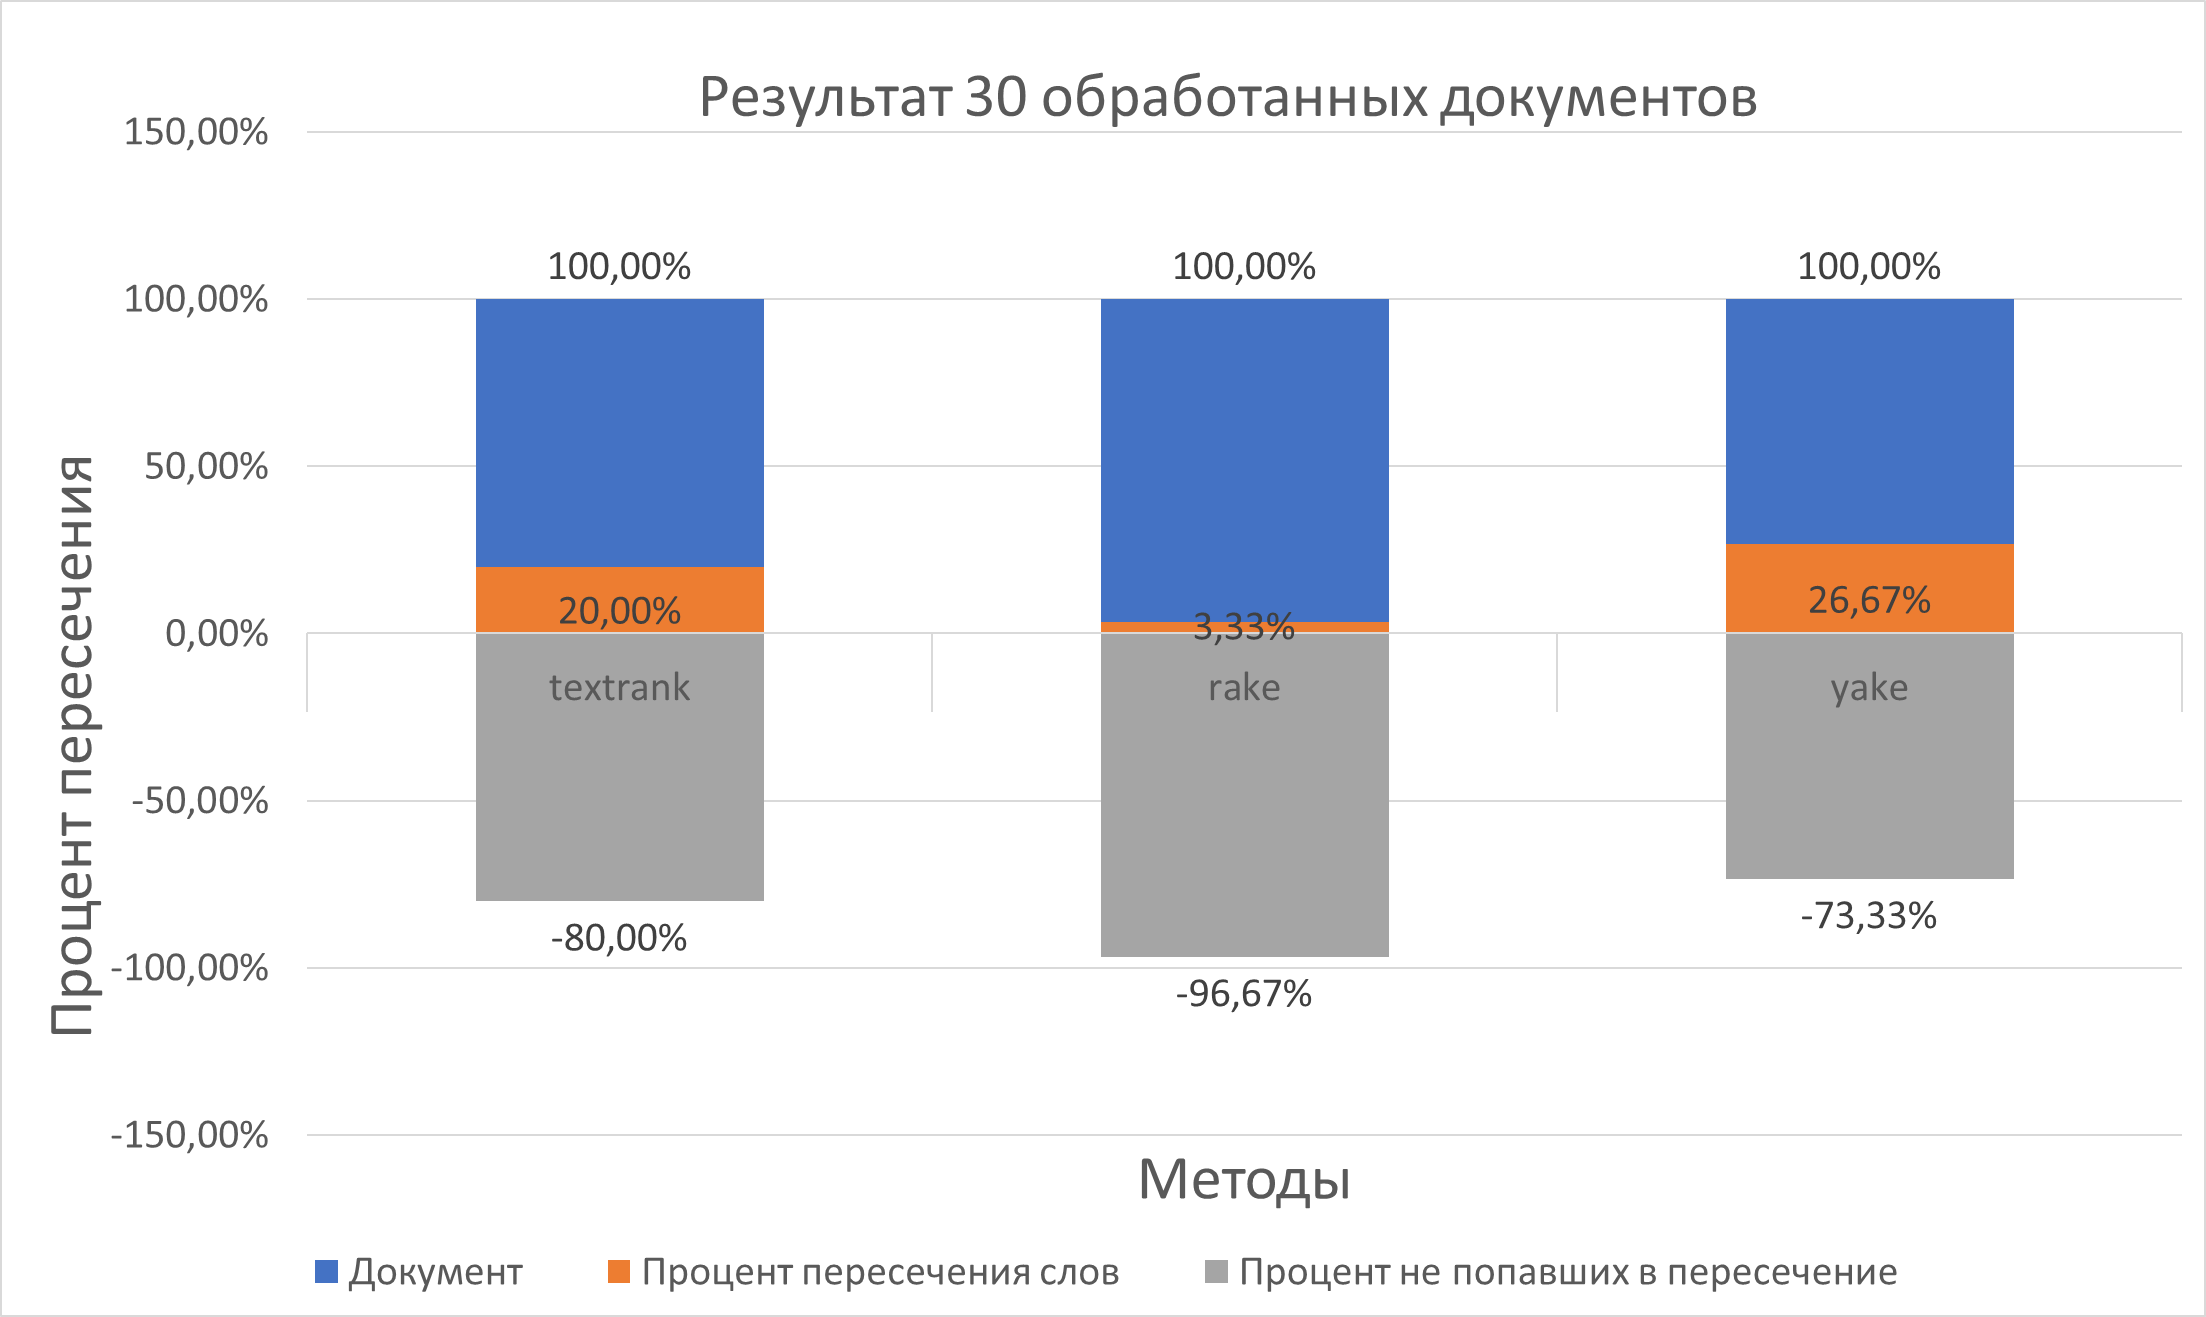
\includegraphics[width=0.7\linewidth]{src/img/experiment/experiment_1_4}
	\caption{Результат обработки 30 документов}
	\label{fig:experiment14}
\end{figure}

По завершению измерений результативности были получены следующие результаты, отображенные в таблице на странице \pageref{table:experiment31}
\begin{table}[!h]
	\begin{tabular}{|c|c|c|c|}
		\hline
		& Yake (mod) & Textrank & Rake \\
		\hline
		Средний \% пересечения & 26.67\% & 20\% & 3.33\% \\
		\hline
		Средний \% не попавших в пересечение & 73.33\% & 80\% & 96.67\% \\
		\hline
	\end{tabular}
	\label{table:experiment31}
	\caption{Результат сравнения методов}
\end{table}
Результатом 30 обработок документа является средний процент пересечения ключевых слов у метода Yake составляет 26.67\% в то время когда у Textrank 20 \% у Rake 3.33%.
Процент ключевых слов не попавших в пересечении у метода Yake составляет 73.33\% у Textrank 80\% а у метода rake составил 96.67\%

\section{Исследование влияния размерности N-грамм на работу метода}
Для проведения данного исследования был выбран документ: "Идентификация личности по фрактальной размерности отпечатков пальцев и системы контроля и управления доступом" \cite{}.

\begin{figure}[!h]
	\centering
	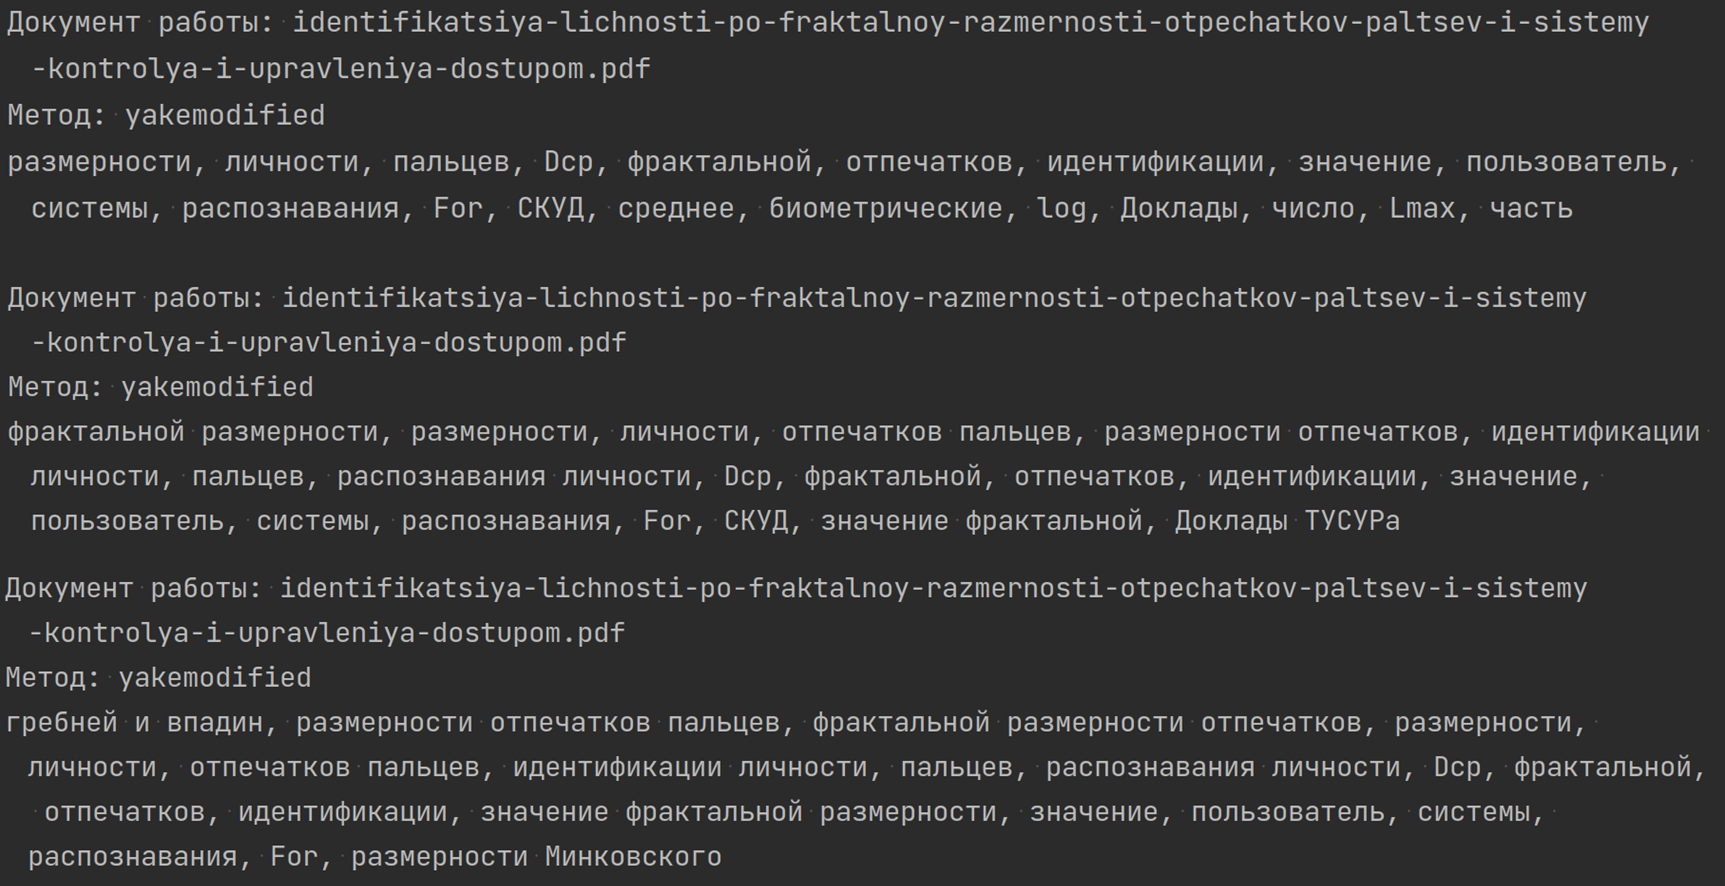
\includegraphics[width=0.7\linewidth]{src/img/experiment/experiment_2_1}
	\caption{Результа извлечения ключевых слов при N = 1 до N = 3}
	\label{fig:experiment21}
\end{figure}

В качестве опорного слова возьмем "пальцев". При N = 2 данное слово преобразуется в словосочетание "отпечатков пальцев". При N = 3 получаем выражением "размерности отпечатков пальцев". На основе этого можно сделать вывод, что метод пригоден для извлечения многокомпонентных ключевых слов.

\section{Вывод}
В результате проведенной исследовательской работы над разработанным решением было установлено, что все требования, поставленные к алгоритму, соблюдены.
Метод способен на извлечение многокомпонентных ключевых слов из документов на русском языке. 

\chapter*{ЗАКЛЮЧЕНИЕ}
\addcontentsline{toc}{chapter}{ЗАКЛЮЧЕНИЕ}
По итогу выполнения работы была выполнена цель по разработке метода автоматического извлечению ключевых слов и словосочетаний из документов на русском языке.
Помимо выше сказанного были проведены исследования, продемонстрировавшие пригодность метода по работе с документами на кириллице.

В процессе выполнения работы:
\begin{enumerate}
	\item проанализирована предметная область и произведена классификация существующих методов по извлечению КС;
	\item разработана архитектура программного обеспечения;
	\item проведена модификация метода и разработаны модули;
	\item произведено исследование получившегося ПО.
\end{enumerate}

Из достоинств полученного метода можно выделить следующее:
\begin{enumerate}
	\item не требует обучения и наличия корпуса текстов;
	\item возможность извлечения n-компонентных ключевых слов;
	\item не использует тезаурусы. 
\end{enumerate}

Из возможных путей развития стоит отметить:
\begin{enumerate}
	\item добавление в предварительную обработку процесса преобразование слов к начальной форме;
	\item добавление автоматического определения языка;
	\item обучение алгоритма определению синонимические терминов;
	\item обучение алгоритма автоматическому определению языка текста.
\end{enumerate}

\makebibliography

\begin{appendices}
	\chapter{}
	\includelisting
	{yakemodified.py}
	{Код модифицированного метода yake}
	\includelisting
	{MainWindow.py}
	{Код контролера}
\end{appendices}

\end{document}